\chapter{Implementierung}
\label{sec:Implementierung}

\section{Einleitung}
Um eine richtige Architektur des Systems auswählen zu können, fassen wir kurz die benötigte Komponenten zusammen:
\begin{itemize}
\item Eine Komponente für Training eines NER-Modells.
\item Eine Komponente für Extraktion von Entitäten aus deutschsprachigen Texten.
\item Ein Filter für ,,unpassende`` Entitäten, der alle Entitäten, die bestimmte Kriterien nicht erfüllen, herausfiltert.
\item Eine Komponente für Verlinkung von extrahierten Entitäten mit den Eigenschaften aus einer Wissensdatenbank.
\item Eine API für Anreicherung von Suchergebnissen.
\end{itemize}

Damit alle aufgelistete Anforderungen im Rahmen dieser Arbeit implementiert werden könnten, muss ein Framework verwendet werden, das eine API für die Arbeit mit semantischen Daten ermöglicht, und folgende Voraussetzungen erfüllt:
\begin{enumerate}
\item Quelltexte des Frameworks müssen frei verfügbar sein, damit die entsprechende Erweiterung implementiert werden könnte.
\item Das Framework muss dem Entwickler die Möglichkeit geben, mehrere Algorithmen für Extraktion von Entitäten gleichzeitig einzusetzen, damit alle im Kapitel ,,Grundlagen`` beschriebene Algorithmen implementiert werden könnten.
\item Das Framework soll dem Entwickler eine REST-API zur Verfügung stellen, mit deren Hilfe auf Funktionen des Systems zugegriffen werden könnte, damit eine Integration mit Drittapplikationen (Siehe Sektion \ref{sec:Problemstellung}) implementiert werden könnte. Die zur Verfügung gestellte REST-API kann dabei von der Anreicherung-API direkt verwendet werden.
\end{enumerate}

Im Rahmen dieser Arbeit wurde als solches Framework Apache Stanbol\footnote{\url{http://stanbol.apache.org/} (Zuletzt abgerufen am 04. November)} ausgewählt. Obwohl es andere Systeme, wie Alchemy API \footnote{\url{http://www.alchemyapi.com/}} gibt, die auch deutsche Sprache unterstützen, hat Stanbol gravierende Vorteile anderen Frameworks gegenüber:
\begin{itemize}
\item Die Quelltexte von Stanbol sind frei verfügbar, was die Entwicklung einer Erweiterung einfacher macht. Im Gegenteil dazu ist Alchemy API ein ,,Black Box`` - es gibt keine Möglichkeit, sich die in diesem Framework verwendete Algorithmen anzugucken oder die zu ändern, es gibt keine Möglichkeit, eigene Anpassungen durchzuführen.
\item Stanbol stellt dem Entwickler eine eingebettete REST-API zur Verfügung, was eine Ankopplung an Drittsysteme erleichtert.
\item Stanbol hat eine modulare Architektur, was bedeutet, dass die in dieser Arbeit benötigte Komponente sich genau so implementieren lassen, wie die beschrieben wurden, als voneinander getrennte Module.
\item Außerdem wird dem Entwickler eine interne Wissensdatenbank zur Verfügung gestellt, was die Benutzung einer getrennter Software für die Implementierung der Verlinkung unnötig macht. 
\end{itemize}
Durch die beschriebene Vorteile erfüllt Apache Stanbol alle im letzten Paragraph erwähnte Bedingungen.

\section{Apache stanbol}
Apache Stanbol stellt dem Entwickler eine Plugin-API zur Verfügung, mit deren Hilfe neue Features wie Extraktion von Entitäten aus deutschen Texten leicht implementiert werden können. Die Liste von verfügbaren Modulen ist auf der Abbildung \ref{fig:komponenten} zusammengefasst.

\begin{figure}[ht]
\centering
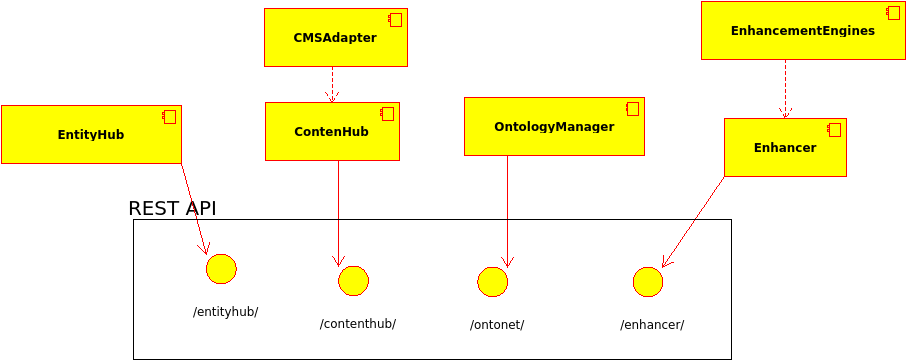
\includegraphics[width=0.6\textwidth]{Bilder/komponenten.png}
\caption{''Komponentendiagramm vom Stanbol''}
\label{fig:komponenten}
\end{figure}

\begin{itemize}
\item \textbf{EntityHub} ist die interne Datenbank, wo die Informationen über Entitäten gespeichert werden. Diese kann sowohl mithilfe von Java API als auch über eine REST-Schnittstelle für die Verlinkung benutzt werden. Als Datenquelle können sowohl ,,Referenced Sites`` (externe Datenquellen die sich auf anderen Maschinen befinden, und auf die EntityHub per Netzwerk zugreift) als auch lokale Indexes verwendet werden. Man kann EntityHub als eine Art von Aggregator betrachten, der mehrere Wissensdatenbanken über eine einheitliche API zur Verfügung stellt. 
\item \textbf{Enhancer} und \textbf{EnhancementEngine} sind die Kernkomponenten von Stanbol, die für die Anreicherung von Texten mit Annotationen zuständig sind.
\item \textbf{OntologyManager} wird, wie sagt der Name, für die Verwaltung von Ontologien zuständig.
\item \textbf{ContentHub} wird für die Integration mit CMS gebraucht und stellt eine Datenbank für das \textit{Content} einer CMS zur Verfügung (nicht für die Entitäten!).
\end{itemize}
Im Rahmen dieser Arbeit werden nur Engines und EntityHub gebraucht, andere Module sind für die Extraktion von Entitäten irrelevant.

\paragraph{}
Die grundlegende Idee, die die Architektur von Stanbol prägt, heißt ,,Pipelining`` - ein Fließband, das mehrere Textverarbeitungsschritte miteinander verknüpft, und eine flexible Konfiguration von Contentanreicherung ermöglicht. Jedes Element dieses Fließbandes wird ,,Engine`` genannt. Von dem Blickwinkel der Architektur wird jedes Engine als eine selbstständige Blackbox implementiert, die am Eingang den Text, der angereichert werden soll, mit den von anderen Engines hinzugefügten Annotationen zusammen, bekommt, und am Ausgang neue Annotationen liefert. 

Die Engines werden in sogenannte Ketten zusammengebunden - der Ausgang von einem Engine wird mit dem Eingang von einem anderen Engine verbunden, und so wird eine virtuelle Kette aufgebaut. Das erste Element in dieser Kette bekommt dabei als Eingang den Text eines mithilfe von einer Suchmaschine gefundenen Snippets, und der Ausgang von dem letzten Element wird zu dem Benutzer geschickt.

Auf der Abbildung \ref{fig:ENGINEPIPELINE} wird der Aufbau der in dieser Arbeit verwendeter Engine-Kette noch einmal grafisch dargestellt.
\begin{figure}[ht]
\centering
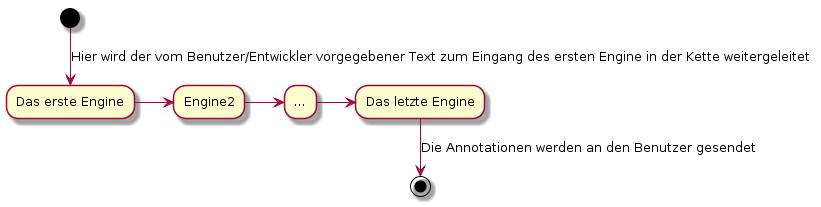
\includegraphics[width=\textwidth]{Bilder/enchancer.png}
\caption{''Graphische Darstellung des Anreicherungspipelines''}
\label{fig:ENGINEPIPELINE}
\end{figure}
Nachdem der Text, der angereichert werden soll, über REST API ausgelesen wurde, werden zuerst rohe Textdaten aus HTML extrahiert, was für Anreicherung von Webseiten notwendig ist. Falls die Daten aber schon im Plaintext gesendet wurden, wird dieser Schritt ignoriert. Danach muss die Sprache des Textes erkannt werden, anhand deren entschieden wird, ob der Text angereichert werden kann. Für die Erkennung der Sprache stellt Stanbol bereits ein Engine \footnote{\url{https://stanbol.apache.org/docs/trunk/components/enhancer/engines/langidengine.html} (zuletzt abgerufen am 10. November)} zur Verfügung.

Falls die Sprache von der Kette unterstützt wird, werden die Sätze und Tokens extrahiert. Die Engines für die Erkennung von Sätzen und Tokens, die deutsche Sprache unterstützen, sind als Standardteil der API verfügbar.

Anschließend können aus dem Text, der vorverarbeitet wurde, Entitäten extrahiert werden. Nach den Extraktion-, Verlinkung- und Filterungsschritten wird der mit Annotationen angereicherte Text über eine REST-Schnittstelle zurückgegeben.

Als Entwickler muss man aber gleich beachten, dass die interne Implementierung von Ketten diese Architektur leider nicht anschaulich abbildet. Wie es auf der Abbildung \ref{fig:REALPIPELINE} zu sehen ist, gibt es intern keine Pipeline - stattdessen wird es für jeden Text, der angereichert werden soll, eine Instanz der Data-Klasse ,,ContentItem`` erzeugt, die zwischen allen Engines der Kette geteilt wird. Die Implementierung eines Engines hat technisch gesehen weder Ein- noch Ausgang, und benutzt stattdessen eine Instanz von ,,ContentItem``, um die Informationen mit anderen Engines auszutauschen. Die Reihenfolge von Elementen in der Engine-Kette bestimmt deswegen nicht, wie die Ein- und Ausgänge von Engines miteinander verbunden werden sollen, sondern die Reihenfolge, in der die Engines ausgeführt werden müssen.

\begin{figure}[ht]
\centering
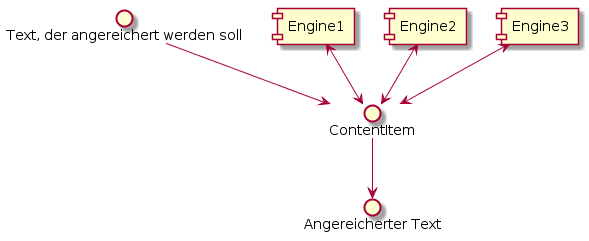
\includegraphics[width=\textwidth]{Bilder/realarch.png}
\caption{''Interne Implementierung einer Engine-Kette''}
\label{fig:REALPIPELINE}
\end{figure}
Der Nachteil solcher Architektur ist, dass mehrere Engines unter Umständen auf dieselbe Instanz von ,,ContentItem`` \textbf{gleichzeitig} zugreifen können, was bei Schreibzugriffen zur Beschädigung von Daten führen kann. Deswegen soll jedes Engine die Instanz von ,,ContentItem`` während des Schreibzugriffs sperren lassen.

Der Vorteil dieser Architektur besteht darin, dass bei Bedarf mehrere Engines parallel für den gleichen Content ausgeführt werden können. Dies kann z. B. dann nützlich sein, wenn es in mehreren Wissensdatenbanken gleichzeitig nach den Informationen über eine Entität gesucht werden muss. Da das ,,ContentItem``-Objekt nur dann mit einem Lock gesperrt werden muss, wenn die Daten \textbf{geschrieben} werden, könnte \textbf{die Suche} in mehreren Wissensdatenbanken parallel durchgeführt werden.

Um sicherstellen zu können, dass nur die Engines, die eine parallele Ausführung unterstützen, parallel gestartet werden, muss der Entwickler in der Konfiguration des Engines explizit eingeben, ob eine parallele Ausführung für das entwickelte Engine möglich ist.

\section{Extraktion von Entitäten} \label{sec:extraktimpl}
Da die Vorverarbeitungsschritte bereits als Teil von Stanbol implementiert sind, ist die Erkennung von Entitäten das erste Modul, das entwickelt werden muss. Die Schritte, die für die Entwicklung eines Engines unternommen werden müssen, lassen sich wie folgt definieren:
\begin{itemize}
\item Ein Engine wird als ein Objekt der Klasse ,,AbstractEnhancementEngine`` implementiert. 
\item Diese Klasse soll dem Framework folgende Methoden zur Verfügung stellen, die die Integration des Engines in eine Enginekette ermöglichen:
\begin{itemize}
\item Eine Aktivierungsmethode, die ein mal beim Start des Engines aufgerufen wird. Diese Methode soll das für das Engine benötigte Modell aus einer Datei laden (ein vortrainiertes SVM-Modell, z. B.).
\item Die Methode, die für den angegebenen Text sagt, ob das Engine diesen Text anreichern kann. Dadurch wird sichergestellt, dass nur die Sprache, die Engine tatsächlich unterstützt, bearbeitet wird.
\item Die Hauptmethode, die für den angegebenen Text Annotationen berechnet.
\end{itemize}
\item Die Ketten, die Engines miteinander verbinden, können sowohl während der Laufzeit als auch vor dem Kompilieren des Systems in einer Konfigurationsdatei definiert werden.
\end{itemize}

\subsection{StanfordNER} \label{subsec:stanfordner}
\paragraph{}
Die erste Anreicherungskette wurde auf Basis von StanfordNER\cite{Jenny/etal:07} aufgebaut. Dieses Framework implementiert das CRF-Algorithmus und stellt ein Modell für die deutsche Sprache zur Verfügung\cite{faruqui10:_training}. Der Nachteil dieses Engines ist, dass es nur ein vortrainiertes Modell zur Verfügung gestellt wird - die Korpora selbst, auf deren Basis ein eigenes Modell trainiert werden könnte, stehen nicht zur Verfügung. Der Vorteil dabei ist, dass es insgesamt zwei vortrainierte Modelle zur Verfügung stehen:

\begin{enumerate}
\item HGC - Huge German Corpus-generalized classifier - dieses Modell wurde auf Texten aus Zeitungen trainiert.
\item deWac - dieser Klassifikator wurde auf Texten aus Internet trainiert.
\end{enumerate}

Dieses Framework stellt außerdem die Möglichkeit zur Verknüpfung von mehreren Modellen miteinander zur Verfügung. Deswegen kann es im Rahmen dieser Arbeit neben dem Austesten von oben genannten Modellen auch ein kombiniertes Modell getestet werden - es ist möglich, dass ein kombiniertes Modell mehr Entitäten im Text finden könnte, andererseits steigt dabei die Wahrscheinlichkeit von False-Positive-Antworten.

Dieses Framework ist auch für die Vorverarbeitung - Zerlegung des Textes in einzelne Sätze und Zerlegung von Sätzen in einzelne Tokens - verantwortlich. Deswegen sind für den auf Stanford-NER basierten Ansatz nur zwei Vorverarbeitung-Engines notwendig:
\begin{enumerate}
\item Tika-Engine für die Extraktion von rohen Textdaten aus HTML.
\item Spracherkennungsmodul, mit deren Hilfe sichergestellt wird, dass die Analyse nur für deutsche Sprache gestartet wird.
\end{enumerate}

Das Klassendiagramm für dieses Engine ist auf der Abbildung \ref{fig:stanfclasses} zu sehen.

\begin{figure}[ht]
\centering
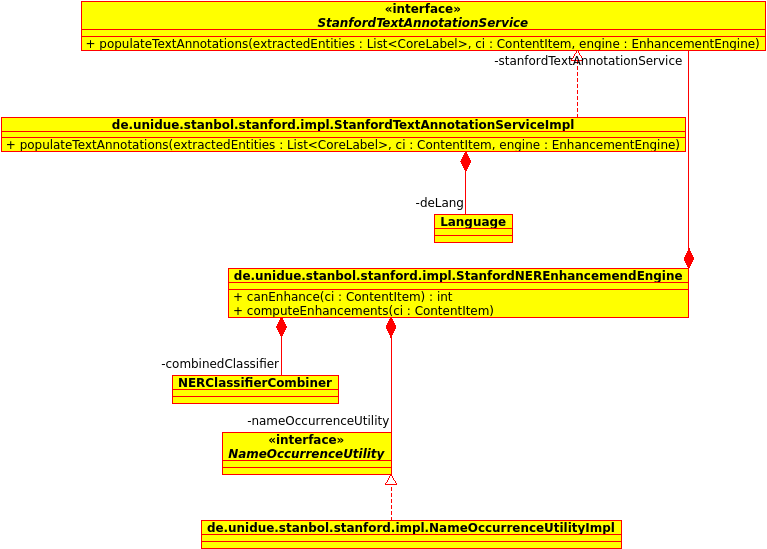
\includegraphics[width=\textwidth]{Bilder/stanford-classes.png}
\caption{''Klassendiagramm  des Stanford-Engines''}
\label{fig:stanfclasses}
\end{figure}
\begin{itemize}
\item Die Klasse \textit{StanfordNEREnhancementEngine} ist die Hauptklasse, die nach den Entitäten im Text sucht.
\item \textit{NERClassifierCombiner} ist die interne Klasse des StanfordNER-Frameworks und stellt die Schnittstelle zum Kombinieren von mehreren NER-Modellen zur Verfügung.
\item \textit{NameOccurenceUtility} ist eine Hilfsklasse, die die Daten zwischen StanfordNER- und Stanbol-Format umwandelt.
\item \textit{StanfordTextAnnotationService} ist ein Hilfsservice, das die vom Engine gefundene Entitäten zum ,,ContentItem`` als Annotationen hinzufügt.
\end{itemize}

\subsection{OpenNLP}
%Beschreibung des OpenNLP-Einsatzes.
Das weitere Algorithmus, das im Rahmen dieser Arbeit verwendet wurde, ist MaximumEntropy. Es wurde als Teil der OpenNLP\footnote{\url{http://opennlp.apache.org/} (Zuletzt abgerufen am 30. Oktober)}-API implementiert. OpenNLP ist ein quelltextoffenes Framework für maschinelle Sprachverarbeitung. Das Framework ist genau wie Stanbol modular aufgebaut, und stellt folgende Funktionalität zur Verfügung:

\begin{itemize}
\item Erkennung von Sätzen. Genau wie für die Extraktion von Entitäten wird für die Satzerkennung ein Maximum-Entropy-Modell verwendet, das vorher trainiert werden muss. Ein Modell für die deutsche Sprache, trainiert auf der Basis von TIGER-Korpus, das in nachfolgendem Kapitel beschrieben ist, ist bereits als Teil des Frameworkes verfügbar.
\item Zerlegung von Sätzen in Tokens, die auf zwei Arten und Weisen durchgeführt werden kann:
\begin{itemize}
\item Die Zerlegung kann ohne vortrainiertes Modell, nur anhand von den in dem Text vorhandenen Leerzeichen, erfolgen.
\item Es kann ein ME-Modell verwendet werden, um Tokens zu erkennen. Der Nachteil dieser Methode ist, dass das Modell zuerst trainiert werden muss, wozu ein Korpus gebraucht wird. Da ein Modell für die Tokenisierung von deutschen Texten als Teil des OpenNLP-Frameworks verfügbar ist, wird im Rahmen dieser Arbeit die modellbasierte Methode verwendet.
\end{itemize}
\item POS-Tagging - die Erkennung und Annotierung von Wortarten - während dieses Vorgangs wird jedem Token eine entsprechende Wortart zugeordnet.
\item Erkennung von Entitäten mithilfe von einem vortrainierten ME-Modell. Hierfür stellt OpenNLP kein vortrainiertes Modell für die deutsche Sprache zur Verfügung.
\end{itemize}

Der Vorteil dieses Engines ist, dass es als Teil vom Stanbol dem Entwickler zur Verfügung steht, und muss deswegen nicht manuell integriert werden. Allerdings müssen die entsprechende ME-Modelle für die Extraktion von deutschsprachigen Entitäten vom Entwickler trainiert werden, worauf in der Sektion \ref{subsec:decor} angegangen wird.

Das Klassendiagramm für das OpenNLP-Engine ist auf der Abbildung \ref{fig:onlpuml} definiert. Es werden insgesamt nur drei Klassen verwendet:
\begin{itemize}
\item Die Basisklasse \textit{NEREngineCore}, die die Extraktion von Entitäten mithilfe vom ME-Algorithmus implementiert.
\item Die Klasse \textit{CustomNERModelEnhancementEngine}, die von der Basisklasse erbt, und für Behandlung von benutzerdefinierten Modellen zuständig ist.
\item Die Konfigurationsklasse \textit{NEREngineConfig}.
\end{itemize}

\begin{figure}[ht]
\centering
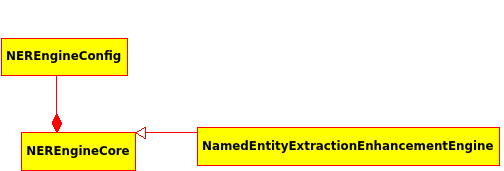
\includegraphics[width=\textwidth]{Bilder/onlp-classes.png}
\caption{''Klassendiagramm des OpenNLP-Engines''}
\label{fig:onlpuml}
\end{figure}

\subsection{MITIE}
\paragraph{}
Der dritte Ansatz, der implementiert werden soll, ist SVM-Algorithmus. Als Basis für diese Unteraufgabe wurde MITIE\footnote{\url{https://github.com/mit-nlp/MITIE} (Zuletzt abgerufen am 03. November)}-Framework ausgewählt. MITIE steht für ,,MIT Information Extraction`` - ein Framework zur Extraktion von Entitäten und zur Erkennung von binären Relationen. Wie erwähnt, verwendet dieses Framework SVM als Basisalgorithmus für Erkennung von Entitäten, und soll deswegen auch bessere Ergebnisse als OpenNLP oder StanfordNER aufzeigen können (siehe Sektion \ref{sec:SVNGRUND}).

Der Aufbau dieses Engines ähnelt sich dem vom Stanford-NER-Engine, und ist auf der Abbildung \ref{fig:mitieclasses} vorgestellt.

\begin{figure}[ht]
\centering
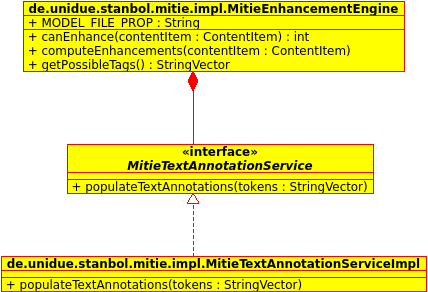
\includegraphics[width=\textwidth]{Bilder/mitie-classes.png}
\caption{''Klassendiagramm  des MITIE-Engines''}
\label{fig:mitieclasses}
\end{figure}
Die Klassen, die in diesem Engine verwendet werden, spielen ähnliche Rollen, wie bei dem Stanford-NER Engine, mit folgender Ausnahme: die Klasse \textit{NamedEntityExtractor}, die für die Extraktion von Entitäten zuständig ist, wird automatisch aus den C++-Quelltexten erzeugt, und nicht manuell entwickelt.

\paragraph{Vor- und Nachteile}
\begin{itemize}
\item Vorteile des MITIE-Frameworks:
\begin{enumerate}
\item Höhere Qualität der Extraktion, im Vergleich zu Maximum Entropy oder CRF.
\item Die Geschwindigkeit der Extraktion ist nicht viel kleiner, als die bei den anderen Engines.
\end{enumerate}
\item Nachteile des MITIE-Engines:
\begin{enumerate}
\item Die Größe des Modells ist im Vergleich zu den ME- oder CRF-Modellen relativ hoch(323 Mb im Vergleich zu 3 Mb für ein OpenNLP-Modell)
\item Das Training eines SVM-Modells kann bis auf mehrere Tage dauern.
\item Ein rein technischer Nachteil - die MITIE-Implementierung ist in C++ geschrieben und ist außerdem nicht thread-sicher, was zu folgenden Einschränkungen führt:
\begin{enumerate}
\item Der Aufruf des Engines muss mit einem Lock gesichert werden, was die Geschwindigkeit bei mehreren Benutzern, die auf das Engine gleichzeitig zugreifen, beeinträchtigt.
\item Jeder Fehler in dem Engine kann potentiell zum Absturz der JVM-Software führen.
\end{enumerate}
\end{enumerate}
\end{itemize}

\subsection{Deutcshe Korpora} \label{subsec:decor}
Nachdem die Engines, die nach den Entitäten in den Texten suchen sollen, entwickelt wurden, müssen die entsprechende NER-Modelle trainiert werden, wie es in der Sektion \ref{sec:trcorpora} beschrieben wurde. Und obwohl fällt dieser Schritt für das auf Stanford-NER basierten Engine komplett aus, da dieses Engine ein vortrainiertes Modell verwendet, müssen für weitere zwei Engines eigene Modelle trainiert werden.

Im Rahmen dieser Arbeit wurden zwei Trainingskoprora verwendet: von den Linguisten erzeugtes TIGER-Korpus und auf Basis von Wikipedia-Artikeln aufgebautes PIG-Korpus. Diese beide Korpora wurden aus folgenden Gründen ausgewählt:
\begin{itemize}
\item TIGER-Korpus wurde ausgewählt, da es das einzige deutschsprachige Korpus mit annotierten Entitäten ist, das frei verfügbar ist und das eine genügende Anzahl von Sätzen(50472 Sätzen) beinhaltet - das vom Sebastian Padó\cite{faruqui10:_training} zur Verfügung gestelltes Korpus ist zwar auch frei verfügbar, beinhaltet aber nur 857 Sätzen, was fürs Training ungenügend ist.
\item Wikipedia wurde als Basis für automatisch aufgebautes Korpus ausgewählt, da die Dumps von Wikipedia frei verfügbar sind und eine große Anzahl von Daten (215841 Sätzen) beinhalten.
\end{itemize}

Für das Training von Modellen für beide Engines (MITIE und OpenNLP) wird dasselbe Datenformat verwendet, das in der Auflistung \ref{lst:TIGEROPENBEISPIEL} beschrieben ist. Dadurch wird erreicht, dass der Code fürs Training von beiden Engines wiederverwendet werden kann.

\lstinputlisting[captionpos=b,label={lst:TIGEROPENBEISPIEL},caption={Ausschnitt aus einem Korpus im OpenNLP-Format.}]{Listings/tiger-opennlp.txt}

\subsubsection{TIGER Korpus}
\paragraph{}
TIGER-Korpus wurde von dem Institut für maschinelle Sprachverarbeitung\cite{brants2004tiger} auf der Basis von Zeitungen aufgebaut, und beinhaltet 50474 Sätzen. Außer markierten Entitäten beinhaltet dieses Korpus auch die Informationen über POS (Part Of Speech - Wortart), Lemma (Infinitiv für Verben oder Nominativ Singular für Substantive) und andere Informationen über die annotierte Tokens, wie Kasus oder Genus. Der Ausschnitt des Korpus findet man in der Auflistung \ref{lst:TIGERBEISPIEL}.

\lstinputlisting[captionpos=b,label={lst:TIGERBEISPIEL},caption={Ausschnitt aus dem TIGER-Korpus. Die Informationen, die in dieser Arbeit nicht gebraucht werden, wurden wegen Platzmangel weggelassen.}]{Listings/tiger-example.txt}
Jeder Satz ist dabei auf einer getrennter Zeile gespeichert, die Tokens werden mit einem Leerzeichen getrennt, und mithilfe von HTML-ähnlichen Tags werden die Entitäten markiert.

\paragraph{}
Das Korpus ist wie folgt aufgebaut:
\begin{itemize}
\item Die Sätze werden mit einer leeren Zeile getrennt.
\item Jeder Token und seine Annotationen werden in einer Zeile geschrieben. Die Spalten werden mit einem Leerzeichen getrennt.
\item Die erste Spalte beinhaltet ID des Tokens, die aus Nummer des Satzes und Nummer des Tokens innerhalb des Satzes besteht.
\item Die zweite Spalte ist der Token selbst, so wie er auch im Satz vorkommt.
\item In der dritten Spalte steht Lemma des Tokens.
\item Die vierte Spalte wird nicht verwendet.
\item Und die fünfte Spalte beinhaltet POS-Tag des Tokens. Falls dieser Tag den Wert \textit{NE} hat, ist das entsprechende Token eine Entität.
\end{itemize}

Der Nachteil dieses Korpus besteht darin, dass es zwischen verschiedenen Klassen von Entitäten nicht unterschieden wird, und die alle die Klasse \textit{NE} (NamedEntity) haben.

\paragraph{}
Die Logik, die für die Umwandlung von TIGER-Korpuseinträgen in das OpenNLP-Format verantwortlich ist, ist in der Auflistung \ref{lst:LOGICOFCONVERTER} zu sehen.
\lstinputlisting[captionpos=b,label={lst:LOGICOFCONVERTER},caption={Ausschnitt aus den Quelltexten des Konverters, der die Logik der Umwandlung beschreibt}]{Listings/tiger-to-onlp.java}
Es wird für jede ununterbrochene Reihenfolge von NE-Markierungen ein OpenNLP-Tag erzeugt, und alle Wörter, die keine Entitäten sind, werden ohne weitere Umwandlung kopiert.

\subsubsection{Wikipedia-basiertes Korpus}
\paragraph{}
Ein manuell aufgebautes Korpus kann nicht immer eingesetzt werden, entweder aus Lizenz- oder Kostengründen. Viele Korpora sind nur für Forschung frei verfügbar, was bedeutet, dass die auf keinen Fall in einem Geschäftsprojekt verwendet werden dürfen. Und ein eigenes Korpus kann nicht immer aufgebaut werden, da dazu die Linguisten eingesetzt werden müssen, die nicht jede Firma zur Verfügung hat, und es kann Monaten dauern, bis ein eigenes Korpus erstellt wurde. Was könnte in diesem Fall unternommen werden?

\paragraph{}
Oliver Grisel\footnote{\url{http://www.nuxeo.com/blog/mining-wikipedia-with-hadoop-and-pig-for-natural-language-processing/} (Zuletzt abgerufen am 20. Oktober)} hat einen interessanten Ansatz zur automatischen Aufbau von einem NER-Korpus vorgeschlagen. Es wird vorgeschlagen, Wikipedia als Textbasis zu nehmen, und die interne Links, die auf andere Wikipedia-Seiten führen, als Entitäten zu markieren. Die Klasse der Entität wird dabei direkt aus der Wikipedia extrahiert. Es soll anschließend ein Korpus aufgebaut werden, auf dessen Basis ein NER-Modell trainiert werden kann. Da Wikipedia auch in deutscher Sprache verfügbar ist, soll dieser Ansatz auch für die Zwecke der vorliegenden Masterarbeit eingesetzt werden können.

\paragraph{}
Für den Aufbau des Korpus wird Apache Pig\footnote{\url{http://pig.apache.org/} (Zuletzt abgerufen am 23. Oktober)} verwendet - ein Framework für Big-Data-Analyse, das eine Skript-Sprache und eine JavaAPI zur Verfügung stellt. Der Aufbau vom Korpus umfasst folgende Schritte:
\begin{enumerate}
\item Zuerst wird der Dump von den Wikipedia-Artikeln heruntergeladen.
\item Danach werden die Listen von Wikipedia-Links und Klassen von Entitäten von DBpedia heruntergeladen. Diese Informationen werden später gebraucht, um jeder Entität in dem erzeugten Korpus eine richtige Entitätsklasse zuordnen zu können.
\item Im dritten Schritt werden aus dem heruntergeladenen Wikipedia-Dump die Links auf interne Wikipedia-Artikel extrahiert, mit der Positionsinformationen zusammen.
\item Danach wird jedem Link, das eine Entität beschreibt, eine entsprechende Entitätsklasse mithilfe von den DBpedia-Daten zugeordnet.
\item Anschließend werden die in vorherigen Schritten gewonnene Informationen in einem Trainingskorpus im OpenNLP-Format zusammengefasst.
\end{enumerate}

\paragraph{} 
Für den Aufbau des Korpus aus deutscher Wikipedia können die Scripts von Oliver Grisel\footnote{\url{https://github.com/tastatur/pignlproc} (Zuletzt abgerufen am 30. Oktober)} genommen werden, die allerdings angepasst werden müssen:
\begin{itemize}
\item Es soll deutsche Dbpedia\footnote{\url{http://de.dbpedia.org/} (Zuletzt abgerufen am 10. Oktober)}, und nicht englische verwendet werden.
\item Es soll deutsches Modell für Satzerkennung eingesetzt werden, und nicht englisches.
\item Das Herunterladen von den Wikipedia- und Dbpediadaten soll automatisiert werden.
\end{itemize}

Der Code, der für die Erzeugung eines Wikipedia-basierten Korpus verantwortlich ist, ist in der Auflistung \ref{app:pigcorpus} repräsentiert.

\paragraph{}
Aber welche Vor- und Nachteile hat eine automatische Erzeugung vom Korpus? Kann das trainierte Modell später auch tatsächlich für sinnvolle Erkennung von Entitäten eingesetzt werden?
\begin{itemize}
\item Vorteile
\begin{itemize}
\item Die Erzeugung vom Korpus braucht höchstens eine Stunde, im Vergleich zu manuell annotierten Korpora.
\item Es werden keine Fachleute gebraucht, um das Korpus zu erzeugen.
\end{itemize}
\item Nachteile
\begin{itemize}
\item Nicht alle interne Links stellen eine Entität dar, und nicht alle Entitäten sind ein Link - als Folge ist die Qualität des Korpus deutlich niedriger, als die von manuell aufgebauten Korpora.
\item Eine sehr niedrige Varianz - alle Wikipedia-Artikel sind in einer mehr oder weniger gleicher Sprache geschrieben, was bedeutet, dass wenn man dem trainierten Modell einen Text zeigt, der sich von einem durchschnittlichen Wikipedia-Artikel deutlich unterscheidet, werden in dem Text höchstwahrscheinlich keine Entitäten gefunden.
\end{itemize}
\end{itemize}

\subsection{Training von Modellen} \label{subsec:TRMODELLS}
Sowohl für OpenNLP als auch für MITIE wird Training von Modellen außerhalb vom Stanbol durchgeführt. Die Ergebnisse werden dabei in den binären Dateien gespeichert, und später von den entsprechenden Engines innerhalb vom Stanbol geladen. Der Grund, warum es so gemacht wurde, ist die Geschwindigkeit des Trainings - wie erwähnt, erfordert Training üblicherweise viel größere Rechnerkapazitäten als die Verwendung von den trainierten Modellen. Das MITIE-Engine braucht z. B. mindestens 24 GB Arbeitsspeicher, und das Training eines Modells dauert bis auf eine Woche. Deswegen wurde Training auf den getrennten Rechnern durchgeführt.

Die Implementierung des Trainings umfasst folgende Schritte: 
\begin{enumerate}
\item Zuerst wird die vorab erzeugte OpenNLP-Training-Datei geladen.
\item Danach wird entweder OpenNLP- oder MITIE-API aufgerufen, um ein ME- oder SVM-Modell auf den im ersten Schritt geladenen Daten zu trainieren.
\item Am Ende wird das erzeugte Modell serialisiert und in einer Datei gespeichert.
\end{enumerate}
Das Training von einem OpenNLP-Modell ist in der Auflistung \ref{app:trainonlp} und von einem MITIE-Modell in der Auflistung \ref{app:trainmitie} beschrieben.

Beim Training von einem MITIE-Modell mithilfe vom Wikipedia-Korpus(PIG) musste noch folgende Anpassung gemacht werden: ursprünglich musste das ganze Korpus (215841 Sätzen) fürs Training verwendet werden, allerdings konnte das Training auf einem Rechner mit 24 GB Arbeitsspeicher nicht abgeschlossen werden, deswegen wurden für MITIE zufällige Sätze aus dem PIG-Korpus ausgewählt (71947 Sätzen), und das Modell wurde auf dieser kleineren Korpusversion trainiert.

\section{Verlinkung und Dereferenzierung von annotierten Entitäten} \label{sec:VERLINKUNGSEC}
\paragraph{}
Nachdem die Entitätserkennung durchgeführt wurde, hat man die Informationen darüber, ob es Entitäten im Text gefunden wurden, die Positionen der gefundenen Entitäten innerhalb des Satzes und optional die Klassen der Entitäten. Die Ontologien, die die Eigenschaften der Entitäten beschreiben, die dem Endbenutzer gezeigt werden müssen, fehlen nach dem Schritt der Erkennung von Entitäten noch. Es müssen noch zwei Schritte durchgeführt werden, bis die Informationen komplett sind - Verlinkung von aus den Suchergebnissen extrahierten Entitäten mit den Entitäten in einer Wissensdatenbank und die Dereferenzierung von Eigenschaften der Entitäten.

Als die Datenquelle für die Verlinkung und Dereferenzierung von Entitäten wird in dieser Arbeit lokaler Index der deutschen DBpedia\cite{auer2007dbpedia} verwendet. DBPedia stellt eine Kopie von Wikipedia zur Verfügung, deren Daten als RDF-Graphen gespeichert werden, und auf die mithilfe von SPARQL zugegriffen werden kann.

Während der Verlinkung von Entitäten wird für jede erkannte Entität eine Suche in einer Wissensdatenbank durchgeführt. Um den Vorgang höchstmöglich zu beschleunigen, soll lokaler Index der verwendeten Wissensdatenbank (EntityHub in Terminologie vom Stanbol) eingesetzt werden. Dieser Index soll vorher aufgebaut werden, und zumindest die Namen der Entitäten beinhalten. Für spätere Schritte ist es aber empfehlenswert, die Eigenschaften von Entitäten zum Index hinzuzufügen, damit die Dereferenzierung so schnell wie möglich ausgeführt werden könnte. Es muss aber beachtet werden, dass Index von realen Wissensdatenbanken wie DBpedia mehr als 20 Gigabytes vom Festplattenspeicher verbrauchen kann, und der Aufbau des Indexes kann mehrere Tage in Anspruch nehmen.

Für die Verlinkung von Entitäten wird Engine ,,EntityLinkingEngine`` verwendet, dessen Aufbau auf der Abbildung \ref{fig:linking} beschrieben ist.

\begin{figure}[ht]
\centering
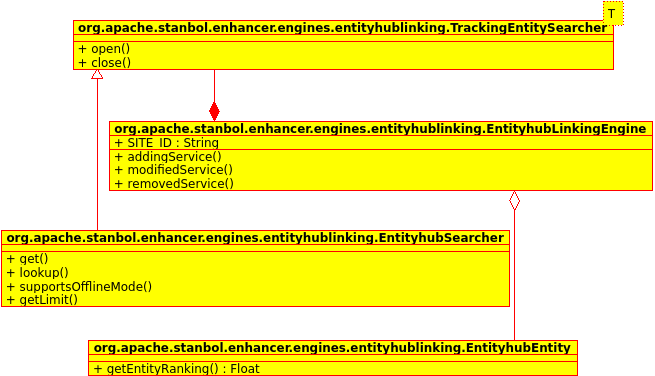
\includegraphics[width=\textwidth]{Bilder/classes-linking.png}
\caption{''Klassendiagramm für EntityLinkingEngine''}
\label{fig:linking}
\end{figure}
\begin{itemize}
\item Die Klasse \textit{EntityHubSearcher}, die Interface \textit{TrackingEntitySearcher} implementiert, ist für die Suche in der Wissensdatenbank zuständig.
\item Die Klasse \textit{EntityHubEntity} stellt eine Entität und ihre Eigenschaften dar. Der Parameter ,,entityRank`` zeigt, wie wichtig die Entität im Vergleich zu anderen Entitäten in der Datenbank ist, was für das Herausfiltern von ,,unpassenden`` Entitäten helfen könnte.
\item \textit{EntityhubLinkingEngine} ist die Hauptklasse, die die Informationen über extrahierte Entitäten verlinkt.
\end{itemize}

Bei der Verlinkung von Entitäten kommt es oft vor, dass die Entitäten, die gefunden wurden, nur Verlinkungen auf andere Entitäten sind, und keine selbstständige Objekte - die Entität ,,CDU`` ist z. B. nur ein Link auf ,,Christlich Demokratische Union Deutschlands``. Solche Entitäten werden während der Verlinkung anhand der Eigenschaft ,,dbo:wikiPageWikiLink`` erkannt, und anstatt dieser Zwischenentität wird als Ergebnis der Verlinkung die referenzierende Entität verwendet.

Um die für den Benutzer relevante Informationen (Eigenschaften von Entitäten) zur Verfügung stellen zu können, müssen diese Eigenschaften aus der Datenbank geladen werden. Dazu könnte man auch direkt auf die entsprechende Schnittstelle zugreifen (http://de.dbpedia.org/resource/ für DBpedia, zum Beispiel), so ein Vorgehen würde aber aus folgenden Gründen ineffektiv sein:
\begin{itemize}
\item Für jede neue Wissensdatenbank muss eine neue Schnittstelle programmiert werden. Das Entityhub stellt dagegen eine universelle API zur Verfügung, die für alle Wissensdatenbanken gleich ist.
\item Im Fall des Ausfalls der externen Datenbank hat das System keinen Zugriff auf die Daten mehr. Dagegen läuft das Entityhub unabhängig von den Drittsystemen. 
\end{itemize}

Deswegen soll auch für die Dereferenzierung das EntityHub eingesetzt werden. Für diesen Zweck wird das Engine \textit{EntityhubDereferenceEngine} eingesetzt, das für jede im Verlinkungsschritt gefundene Entität alle verfügbare Eigenschaften zu dem Anreicherungsergebnis hinzufügt. Das Klassendiagramm für dieses Engine ist auf der Abbildung \ref{fig:deref} zu sehen. 

\begin{figure}[ht]
\centering
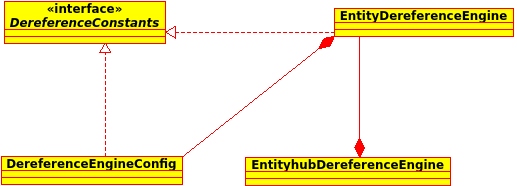
\includegraphics[width=\textwidth]{Bilder/deref-uml.png}
\caption{''UML-Klassendiagramm für EntityhubDereferenceEngine''}
\label{fig:deref}
\end{figure}
Die Klasse \textit{EntityDereferenceEngine} ist die Hauptklasse, die für die Dereferenzierung zuständig ist, und die die Eingabedaten mit entsprechenden Annotationen anreichert. Diese Klasse verwendet zwei Konfigurationsklassen \textit{DereferenceEngineConfig} und \textit{DereferenceConstants}, die die verfügbare Indexe von den Wissensdatenbanken und andere Einstellungen definieren. Die Klasse \textit{EntityhubDereferenceEngine} stellt eine Abstraktion zur EntityHub-API zur Verfügung.

\section{Herausfilterung von für den Benutzer irrelevanten Entitäten}
Wie in der Aufgabenstellung (\ref{sec:Aufgabenstellung}) gesagt wurde, müssen nur relevante Entitäten dem Benutzer angezeigt werden, damit der Benutzer sich nicht verwirrend fühlt. Die beste Lösung dieses Problems wäre eventuell eine semantische Analyse der Benutzeranfrage, und ein Matching von Entitäten mit den Ergebnissen solcher Analyse, aber wegen Zeitmangel und einem zu großen Aufwand, der außer Rahmen dieser Masterarbeit stünde, konnte diese Lösung nicht implementiert werden. Statdessen werden folgende Gewichte verwendet, um zu entscheiden, ob eine Entität wichtig genug ist:
\begin{itemize}
\item Das Gewicht der Entität innerhalb des EntityHubs verwendet, das anhand von Anzahl der Wikipedia-Links, die auf die Entität zeigen, festgesetzt wird. Wert ,,1`` entspricht dabei dem höchstmöglichen und ,,0`` dem kleinstmöglichen Gewicht.
\item Das ,,Sicherheitswert`` (Confidence) der extrahierten Entität - wie hoch ist die Wahrscheinlichkeit $p(y|x)$ (wie in der Sektion \ref{subsec:crftheory} beschrieben), dass das Wort $x$ eine Entität der Klasse $y$ ist.
\end{itemize}

Das Engine, das diesen Filter implementiert, besteht nur aus einer Klasse, die schrittweise überprüft ob die Confidence- und Rank-Werte kleiner als in einer Konfigurationsdatei vordefinierte Schwellwerte sind. Falls ein von den beiden Werten kleiner als Schwellwert ist, wird die Entität aus der Liste von Ergebnissen gelöscht.

Die Schwellwerte für beide Filter (0.7 für Confidence und 0.2 für den Rank) wurden nach manuellem Austesten von Engines anhand persönlichen Erfahrungen des Entwicklers ausgewählt.

\section{API f{\"{u}}r Anreicherung von Suchergebnissen}
\paragraph{}
Um dem Endentwickler die Anreicherung von Suchergebnissen so einfach wie möglich zu machen, wurde eine API entwickelt, die direkt an ein beliebiges Java-Projekt als eine Bibliothek angebunden werden kann. Diese Bibliothek wird auch später in der Evaluierung verwendet. Es wurde eine Abstraktionsschicht hinzugefügt, die die Aufrufe der REST-Schnittstelle von Stanbol hinter der Klientklasse verbirgt. Der Entwickler soll nur die Liste von Suchsnippets an API übergeben, für die Verbindungaufbau zum Stanbol und Parsing der Antwort des Servers ist API verantwortlich. Die Beschreibung der API-Schnittstelle, die für den Entwickler sichtbar ist, findet man in der Auflistung \ref{lst:APISCHNITSTELLE}. 

Als Eingabedaten übergibt man die Liste von URLs gefundenen Webseiten mit dazugehörigen Texten von Snippets zusammen, und als Ausgabe bekommt man für jede URL die Liste von gefundenen Entitäten. Da in Rahmen dieser Arbeit mehr verschiedenen Engineketten implementiert wurden, muss der Name der erwünschten Kette miteingegeben werden.

Die API wurde außerdem so entworfen, dass bei Bedarf nicht nur Stanbol, sondern jedes beliebiges System als Backend verwendet werden kann - für jedes neues Backend muss nur die Klasse ,,EnhancementClient`` abgeleitet werden, und in der abgeleiteten Klasse die Schnitstelle zum neuen System implementiert werden. Gegebenfalls sollen auch neue Konverter geschrieben werden, falls Backend keine RDF-Daten liefert, und eigenes Datenformat verwendet.

Eine UML-Klassendiagramm für die Stanbol-API ist auf der Abbildung \ref{fig:apiuml} zu sehen. Es soll beachtet werden, dass die Schnitstelle zur Suchmaschine absichtlich außer Acht gelassen wurde - um die API so generisch wie möglich zu gestalten, wird die Anbindung an Suchmaschine dem Entwickler, der die API verwendet, überlassen. 

\begin{figure}[ht]
\centering
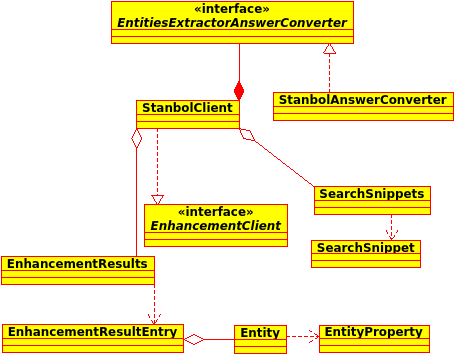
\includegraphics[width=\textwidth]{Bilder/apiuml.png}
\caption{''Struktur der Stanbol-API''}
\label{fig:apiuml}
\end{figure}
\begin{itemize}
\item Die Klasse \textit{StanbolClient} implementiert das Interface \textit{EnhancementClient}, und spielt die Rolle der Hauptklasse für die Konversation mit Stanbol.
\item \textit{StanbolAnswerConverter} umwandelt die Antwort des Stanbol-Servers (RDF) in das interne API-Format:
\begin{itemize}
\item Die Klasse \textit{EnhancementResults}, die als ein Container für gefundene Entitäten dient.
\item Die Klasse \textit{EnhancementResultEntry}, die die  Ergebnisse der Extraktion für eine bestimmte Webseite zusammenfasst.
\item \textit{Entity}, die eine Entität mit den Parametern zusammen (als eine Liste von \textit{EntityProperty}) darstellt.
\end{itemize}
\item Die Klassen \textit{SearchSnippets} und \textit{SearchSnippet} werden für die Zwischenspeicherung von den Snippets und URLs, die eine Suchmaschine geliefert hat, verwendet. Die Schnittstelle zu der Suchmaschine wird von dem Entwickler implementiert.
\end{itemize}